\chapter{Prestazioni}\label{cap:prestazioni}

Le prestazioni del software sono state testate analizzando le note suonate da una chitarra semiacustica accordata con un accordatore professionale di precisione un cent.
I risultati offerti dal software sviluppato sono conformi alle attese desiderate.
L'unico inconveniente risulta essere una leggera polarizzazione in positivo di circa 0.8 Hz della frequenza identificata per ciascuna nota.
Questo difetto, dovuto alle approssimazioni realizzate nei vari passi dell'algoritmo, può essere facilmente corretto, vista la sua natura sistematica.
La figura \ref{fig:accordatore_in_funzione} mostra questo fenomeno.
Come si può vedere, l'indicatore nero risulta essere leggermente spostato a destra rispetto alla frequenza centrale. 

\begin{figure}[h]
  \begin{center} 
    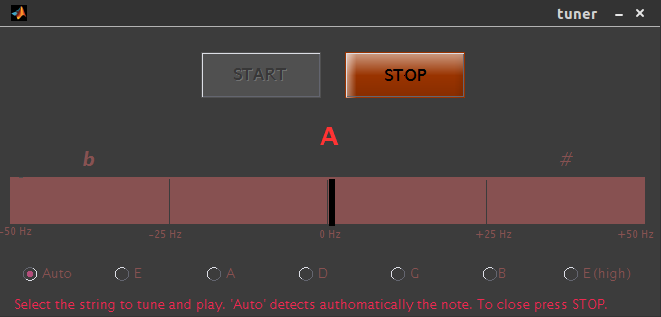
\includegraphics[width=\textwidth*\real{0.8}]{images/ch_08/prestazioni.png}
  \end{center} 
  \caption{\textit{Accordatore in funzione mentre accorda un LA a frequenza 110 Hz. Come si può notare, c'è una leggero spostamento a destra dovuto all'errore sistematico.}}  
  \label{fig:accordatore_in_funzione}
\end{figure}

Un altro fattore che può falsare l'operazione di accordatura è la presenza di disturbi a elevata intensità oppure a bassa intensità ma vicini al microfono. 
In questo caso, infatti, sono presenti delle frequenze aggiuntive che, se comprese nel range [40, 800] Hz, possono essere rilevate come frequenze fondamentali dal software.
La soglia introdotta per distinguere il rumore dalla nota, descritta nella sezione \ref{cap:interpolazione}, risulta essere inutile per questi fenomeni, in quanto, essendo anch'essi dotati di una frequenza fondamentale, presentano un picco ad alta intensità nella funzione prodotto. 
Dal momento che disturbi di questo tipo possono presentarsi a qualsiasi frequenza, risulta impossibile definire un filtro per ridurli. 
Si è quindi deciso di non gestirli.
Anche l'accordatore professionale utilizzato come test, del resto, riconosce le frequenze di questi disturbi.
 
La precisione dell'accordatore professionale, di 1 cent, risulta essere maggiore rispetto a quella del software sviluppato, che nel migliore dei casi, grazie all'interpolazione raggiunge valori di 0,5 Hz.
La relazione logaritmica che lega cent e frequenza, descritta nella formula \ref{formula:cent}, mostra come la precisione raggiunta vari tra i 10 cent a frequenza 82.4 Hz e i 2.62 cent a frequenza di 329.6 Hz.

\begin{equation}\label{formula:cent}
		\Delta_{f_2-f_1} cent = 1200 \log_2 \left( f_2/f_1 \right)
	\end{equation} 

La divisione in cent riflette la modalità di percezione delle frequenze da parte del sistema uditivo umano, di conseguenza, risulta essere una migliore unità di misura per la valutazione della precisione di uno strumento come un accordatore.

Utilizzare una precisione in cent costante, richiede l'utilizzo di una scala logaritmica per l'asse delle frequenze.
Ciò significa sostituire la trasformata di fourier discreta, che utilizza un numero di campioni costante tra frequenze successive, con altre trasformate e, di conseguenza, l'implementazione di un altro algoritmo per il rilevamento della frequenza fondamentale delle note.
L'utilizzo di questo tipo di trasformate non è oggetto di questo lavoro.

 

